

\documentclass[12pt,a4paper]{report}
\usepackage[utf8]{inputenc}
\usepackage[T1]{fontenc}
\usepackage[british]{babel}

\usepackage{amsmath}
\usepackage{amsfonts}
\usepackage{amssymb}
\usepackage{makeidx}
\usepackage{graphicx}
\usepackage{float}
\usepackage[hidelinks]{hyperref}

\usepackage{listings}
\usepackage{color}
\usepackage{url}

\definecolor{dkgreen}{rgb}{0,0.6,0}
\definecolor{gray}{rgb}{0.5,0.5,0.5}
\definecolor{mauve}{rgb}{0.58,0,0.82}

\lstset{frame=tb,
  language=python,
  aboveskip=3mm,
  belowskip=3mm,
  showstringspaces=false,
  columns=flexible,
  basicstyle={\small\ttfamily},
  numbers=none,
  numberstyle=\tiny\color{gray},
  keywordstyle=\color{blue},
  commentstyle=\color{dkgreen},
  stringstyle=\color{mauve},
  breaklines=true,
  breakatwhitespace=true,
  tabsize=3
}



\title{Individual - Architecture Recovery}
\author{ (Nicklas Jeppesen) \\ Course code: KSSOARC2KU}
\date{May 9, 2024}



\begin{document}
	\maketitle
    \tableofcontents
    %\listoffigures

    
    
    \chapter{Introduction}
    The goal for this project is create a Static Analysis of the code base: https://github.com/zeeguu/API. 
    Where the goal should be to be able to take a given function and create a sequence diagram from the methods. 


    \section{Real work life motivation}
    Why this project? why is this usefull and and why static analysis instead of dynamic analysis? 
    
    Motivation from this project, came by when I got a new job where I had to maintain an existing relative large code base, where the code base was part of a eco-system, of multiple systems, where the system could get a request from another system, 
    
    and in the process of handling thar request performing other request to other system, and to then return a response. There didnt exists documentation that explain every single workflow, so to maintain and finding bugs became very hard. The idea was then, what if a system, could crossing systems create a sequence diagram, to virsualize the dependency of the other system. Now micro-services and monolith distributed system has become more popular, so this idea might be usefull for micro-services or monolith distributed systems. 
    This report take the first step on this journey, and try to create a static analyzer which can analyze a single request method to create a sequence diagram from it, in the programming langueage python.

    \subsection*{Why static analyze and not dynamic analyzer?}
    Its well known static analyzer have serveral limitation that danamic analyser dont have, for this it can be difficuilt to determine dead code, wheter it used or not, also if you have implementeted the factory patterns in your code, it hard to say, if you have code that is never executed. So Dynamic code seems to be a better options. Now in my real work case. I had two issues to. 

    first, I was not able to run the program local on my machine, because it needed specific installations files and licence, it was not possible. Even then, we had serveres where the systeem was installed, but then the second problem occur. It needed specific knowledge to trigger a given request in the system, from another system, that I didnt had, and required a colleage. These are the motivation for using a static analyzer, that can analyse not running code, to do reverse engiernering to get an overview of the system. lastly, dynamic analyze is easier in some language than others like it easy in python, but more challenging in languene like java. Where statical analyze does not depend on built in function in the langues.


    \chapter{Methodology}
    
    \section{Tools}
    to creat this project. First this project used to provided from to colab pynb file. Thereafter it used the knowledge about dynamic analysis, and static and dynamic analyzer. To actual analyse the non running code, rich set of regex function was needed to be developered in the progress, for the following reason: 
    \begin{itemize}
        \item Used to extract the imported modules in a file, first inspired by the provided code, but later modified. 
        \item regex is also used to get a list of all functions definiton in a file, used later to figure out what module/file a function call in a function is comming from. 
        \item Used to extract a function body from a string file, and a function name, to analyze. 
        \item regex pattern matching is also used to get a list of function called in a function, for further analysis. 
    \end{itemize}
    
    \subsection{Creating the sequence diagram}
    For drawing the sequence diagram, I use a third party tool called 
     \href{https://github.com/mermaid-js/mermaid-cli}{mermaid-cli}, my code create a string that this tool can transform into a sequence diagram. 



    \chapter{Results}

    \section{what the code provide}
    By providing a filepath as string and function name to the system, it output a png file naming the provided function name containing the the sequence diagram of function. The sequence diagram module names as object, that is because sometimes a file can import a function from a module and not a class, so safe choice is to name the object as the module, and then horientizal line as the function.
   
   
    \section{workflow}
     So how does the work really work? 
    In the Static\_analysis.ipynb file, I have defined, a function called masterFunction, that take a function name and a path to the python file. First the masterFunction get the content of the python file, thereafter it get the function body as a string. thereafter it a list of called functions in the input function,
    
    Then it get a list of all imported modules that are used in the file. Thereafter it get a list of strings in the format <modulename>;<function\_nane>, where all the functions name are the called function in the methods, that are defined inside zeeguu project. Thereafter it return this list. After that, a function named "createMermaid" take that list and conert into a string, that mermaid-cli can understand at transform into a sequence diagram. Lastly, with the mermaid-cli string, function "generate\_sequence\_diagram" are called to transform this string to a sequence diagram, and then a png file is created with the sequence diagram, with the filename of the start function. 


    


    \chapter{Discussion}

    \section{Challenges that I did not expect when starting}

    There was several surprises/challenges I faces, when started on this project, one that is worth of mention is: 

    \subsection{Filename not equal module name}
    One challenge, I didnt expect, when I started this project, was that the imported module, might not be equal to the filename. 
    so to be able to extract a filepath from its module name, became very challenges, and I had the check the init.py file, to search for the correct name, and then again try to find the file name. 

    \section{General limitation of Static analys}

    \section{Limitation for this codebase}
    This project has in some way, ended by becomming a kind of a parser, that can detext code snippet, so to make this project not explored, I had to limit some kind of general code snippet, that python normal can accept, but this code cannot, and these limitation are the following: 

    \subsection{import from new line}
    The example below, shows an example, that my project cannnot handle, because of the use of parantes and new line to import modules. This is one of the limitations I have to live with for now.

    \begin{lstlisting}
        #file: zeeguu/api/endpoints/activity_tracking.py
        from zeeguu.core.user_activity_hooks.article_interaction_hooks import (
            distill_article_interactions,
        )
        \end{lstlisting}


    To fix this issue, I change the code the the import module(s) is on a single line, which my code can handle. as shown below. 

        \begin{lstlisting}
            #file: zeeguu/api/endpoints/activity_tracking.py
             from <path> import distill_article_interactions
        \end{lstlisting}
    
    \subsection{import is not starting of the file}
    another issue I found, was if module is imported in the middle of the file, in a block, then the analyzer cannot register that, like the following issue: 
    \begin{lstlisting}
    #file: zeeguu/api/endpoints/activity_tracking.py, line 41
        if request.form.get("event") == "AUDIO_EXP":
            from zeeguu.core.emailer.zeeguu_mailer import ZeeguuMailer

            ZeeguuMailer.notify_audio_experiment(request.form, flask.g.user)
    \end{lstlisting}
    if the if statement becomes true, then this function call wont be registered, because the import module, was not registered. 
    i change this file too, so I added the from-import code in the top of the file, with the rest, and then, it was registered. 

    \section{Further development} 

    First thing is to correct the already found issues in the discussion section, This would be the first task. 
    Second, With the known knowledge, it could be great to expend this project, so it could have access to multiple code bases/microservices so it would be able to create sequences diagrams for a kubernetes/docker swarm network. third, to be able to create a deeper code anlyzer, that either can anlyze multiple code bases, or go deeper, intil other methods call, one solution could be to create a tree structure, where the root node, could be the first method, and each sub node, could be method calls in the methods, that calls methods either from the code base, or other code base we wnat to examinate, so we dont get system code into our tree. There from that tree, it could be possible to draw a sequence diagram, where each node could hold information about, codebase, module path, ect. 


    \chapter{Time allocation}

    Coding: 80\% \newline
    Writing report: 10\%


    \chapter{Github}

    \url{https://github.com/nicklasjeppesen/software_individual_report}
    
    \appendix
    \chapter{Appendix Figures}

    \begin{figure}[H]
        \centering
        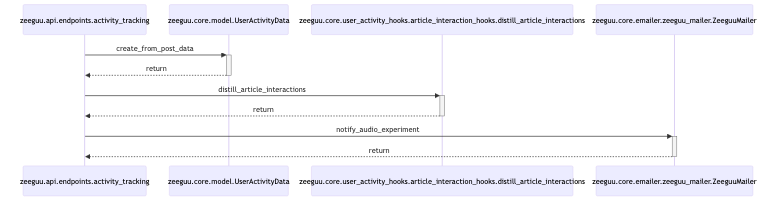
\includegraphics[scale=0.45]{upload_user_activity_data.png}
        \caption{Methods call for method \text{"upload\_user\_activity\_data"} in \text{"activity\_tracking.py"} }
        \label{upload_user_activity}
    \end{figure}
   
    %\paragraph{} Something here?





    \begin{thebibliography}{9}
        
        \bibitem{bl}Google colab code, url: \url{https://colab.research.google.com/drive/1oe_TV7936Zmmzbbgq8rzqFpxYPX7SQHP#scrollTo=0ruTtX88Tb-w}, (accessed: 09.05.2024).
        
        \bibitem{bl}Mermaid-cli: \url{https://github.com/mermaid-js/mermaid-cli}, (accessed: 09.05.2024).
       
        \bibitem{bl}reconstruction part 1: \url{https://github.com/mircealungu/reconstruction/blob/master/1_Introduction.md}, (accessed: 09.05.2024).
        \bibitem{bl}reconstruction part 4, dynamic analysis: \url{https://github.com/mircealungu/reconstruction/blob/master/4_Dynamic_Analysis.md}, (accessed: 09.05.2024).
       
        \bibitem{bl}Dynamic analysis, older material, but have other great examples of issues with static analysis: \url{https://github.com/mircealungu/reconstruction/blob/master/materials/Dynamic_Analysis.md}, (accessed: 09.05.2024).
       
    
    \end{thebibliography}
    

   
    
  
\end{document}


